\section{Evaluation}
\label{sec:eval}

The goal of our large-scale study is to understand how \unsafe{} is used in open-source projects, and what the implications of this on the security of Go applications are. 
To achieve this, we answer the following research questions:

\begin{enumerate}[leftmargin=*,label={RQ\arabic*}]
    \item How many projects use \unsafe{} in Go code in their application? \label{rq:prevalApp}
    \item How many projects introduce \unsafe{} through their dependencies? \label{rq:prevalDeps}
    \item How deep in the import stack are the most imported \unsafe{} code packages? \label{rq:depsDepth}
    \item Which \unsafe{} keywords are used most? \label{rq:distTypes}
    \item What \unsafe{} operations are used in practice, and what is their goal? \label{rq:purpose}
\end{enumerate}

%Figure~\ref{fig:study-overview} provides an overview of our study methodology.
%\begin{figure}[ht]
    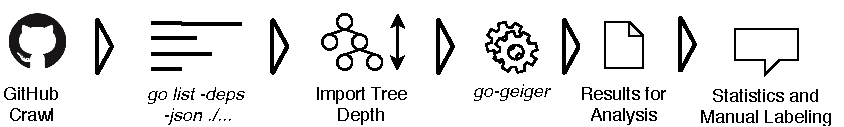
\includegraphics[width=\textwidth]{assets/figures/study-methodology.pdf}
    \caption{Overview of our Study Methodology}
    \label{fig:study-methodology}
\end{figure}


To answer these research questions we first describe our evaluation data set and then provide in-depth analyses of how prevalent \unsafe{} is in the wild, in which way and why it is used in our test data set.
Our evaluation scripts as well as the results are available online\footnote{\todo{Provide link to our paper repository}} for further research.


%% included here for manual positioning one page earlier. Belongs to next section, reposition if needed
\begin{figure*}[!t]
    \vspace{2mm}
    \centering
    %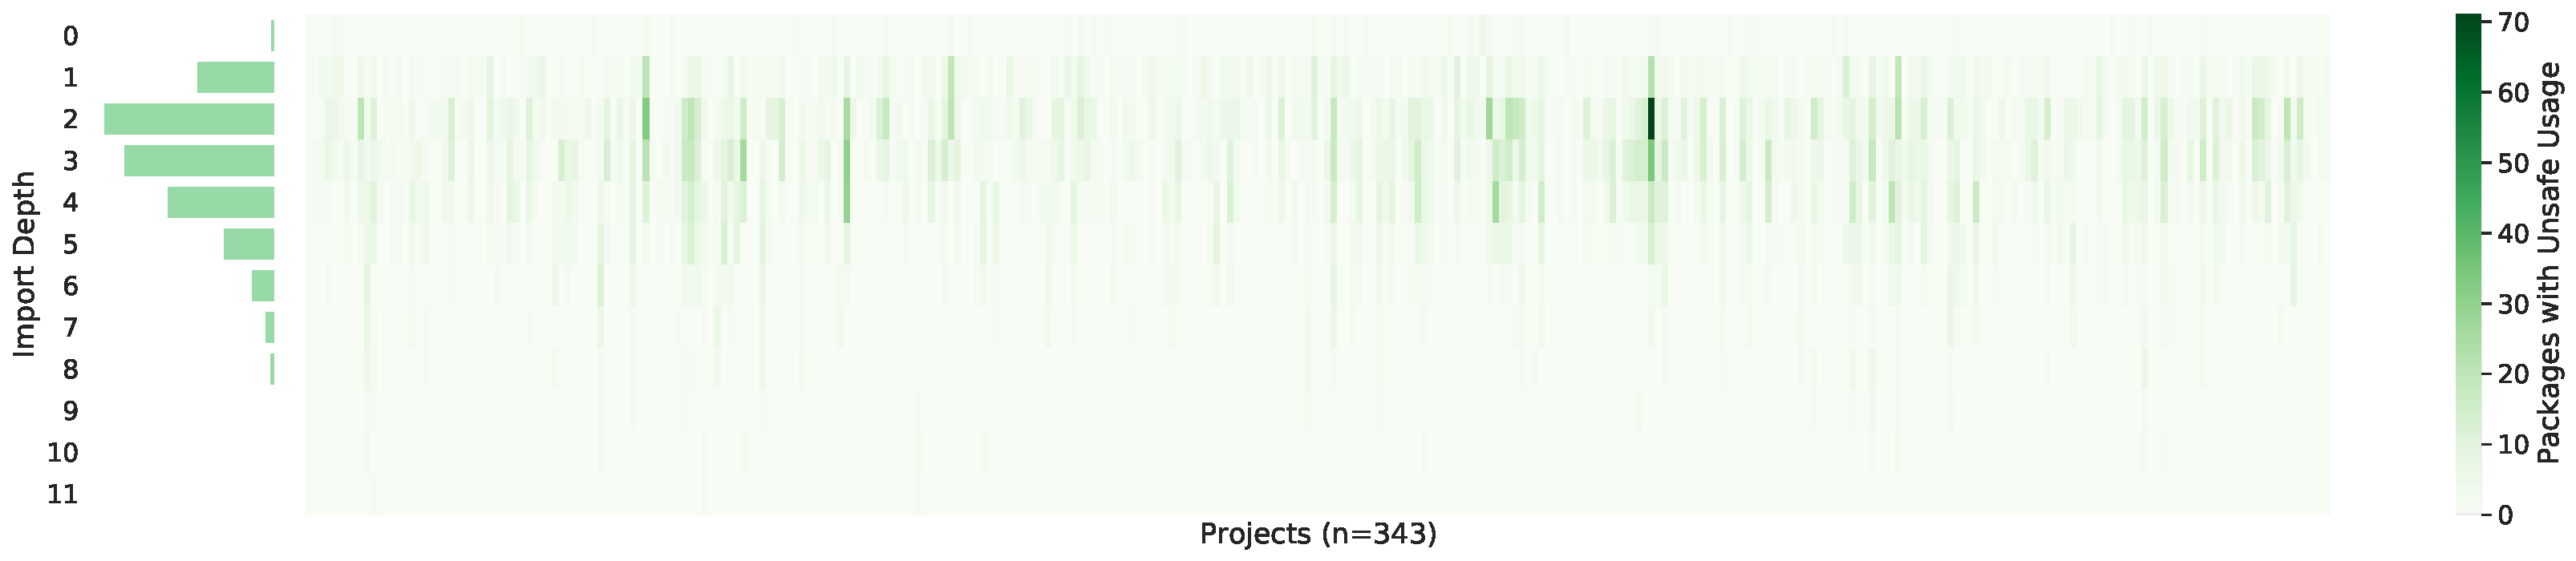
\includegraphics[width=\textwidth]{gfx/figures/unsafe-import-depth.pdf}
    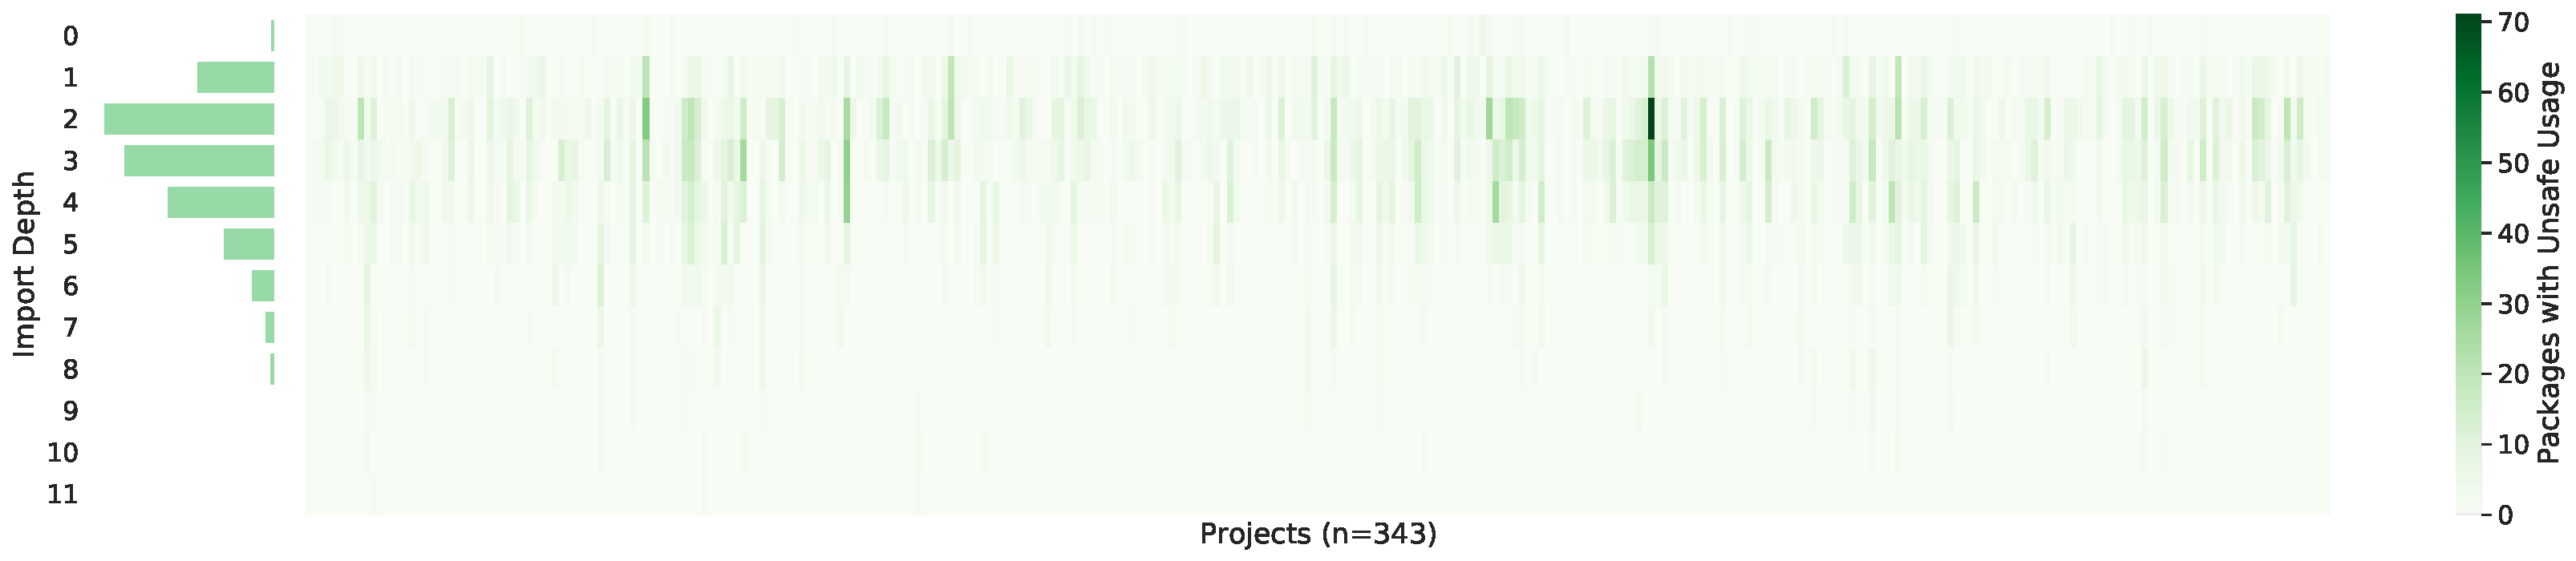
\includegraphics[width=.9\textwidth]{gfx/figures/unsafe-import-depth.pdf}
    \caption{Import Depth of Unsafe Packages. Unsafe packages are around a depth of \averageUnsafeImportDepth{} (sd=\stdUnsafeImportDepth{})}
    \label{fig:unsafe-import-depth}
    %\vspace{-10pt}
\end{figure*}



\subsection{Data Set}

To answer our research questions, we created a data set of open-source Go code available on GitHub.
As our research is focused on projects, we decide to crawl the \initalProjs{} most-stared Go projects available on GitHub. 
To further understand the influence of the dependencies, we selected the applications supporting \textit{go modules}.
With the introduction of Go \checkNum{1.13}, \textit{go modules}\footnote{\url{https://blog.golang.org/using-go-modules}} are the way to include dependencies within a Go application with the help of the Go tool chain. 
Unfortunately, \withoutModules{} of the projects did not yet support Go modules and we had to exclude them.
We further had to remove \notCompiled{} projects as we couldn't compile those.
As a result, we end up with \projsAnalyzed{} top-rated Go projects collected from GitHub.
Our projects have between 72,988 and 3,075 stars, with an average of 7,860 and median of 5,345, thus we analyze a subset of very popular projects.

We use the Go tool chain to identify the root module of every project, that is the module that is defined by the top-level \textit{go.mod} file in the project.
Then, we enumerate the transitive dependency packages of the project, and build the import tree. Using this import tree, we can identify the import depth as minimum depth in the tree for each package.
For each package, we then use \toolUsage{} to find usages of \unsafe{} and save all findings including a context of some code lines for further inspection into CSV files.


\subsection{Unsafe Usages in Projects and Dependencies}

We answer the research questions of how many projects use \unsafe{} in Go code in their application (\ref{rq:prevalApp}), how many projects introduce \unsafe{} through their dependencies (\ref{rq:prevalDeps}), and how deep in the import stack are the most imported \unsafe{} code packages (\ref{rq:depsDepth})?
Our data shows that  \checkNum{131} (\checkNum{38.19\%}) projects have at least one \unsafe{} usage within the project code.

\begin{tcolorbox}
Answer to \ref{rq:prevalApp}: About \checkNum{38\%} of projects directly contain at least one \unsafe{} usage.
\end{tcolorbox}

We find \checkNum{3,388} of \checkNum{62,025} (\checkNum{5.46\%}) transitively imported packages use \unsafe{}. This includes the standard library, of which \checkNum{33} or \checkNum{186} (\checkNum{17.74\%}) use \unsafe{}.
There are \checkNum{299} (\checkNum{87.17\%}) projects that have at least one direct dependency to a package that has $\geq 1$ unsafe dependency, however for this number we counted only packages belonging to the project's root module as first-party project code. \jl{Might be wrong numbers}
If a project is split into several modules that all should be logically viewed as first-party project code, they will inflate this number.
Finally, \checkNum{312} (\checkNum{90.96\%}) projects have at least one transitive dependency with \unsafe{} usages anywhere in the import stack.
These numbers do not include the Go standard library.
Since all projects include the Go runtime, and the runtime uses \unsafe{}, there would otherwise simply be \checkNum{100\%} of projects that transitively include \unsafe{}.
This would however be less meaningful, as we assume the Go standard library is thoroughly audited and safe to use.

\begin{tcolorbox}
Answer to \ref{rq:prevalDeps}: All projects import the Go runtime, which contains \unsafe{}. Other than that, about \checkNum{91\%} of projects transitively import at least one dependency that contains \unsafe{}.
\end{tcolorbox}

Figure~\ref{fig:unsafe-import-depth} shows the number of packages with at least one \unsafe{} usage by its import depth for every project at its own, alongside the distribution for all projects combined.
We see that most of the packages are imported early in the import stack with an average import depth of \averageUnsafeImportDepth (standard deviation of \stdUnsafeImportDepth).
Therefore, these packages can be manually found and evaluated with tolerable effort.

\begin{tcolorbox}
Answer to \ref{rq:depsDepth}: Most of imported packages that contain \unsafe{} usages are around a depth of \checkNum{3} in the package import tree (sd=\checkNum{1.6}).
\end{tcolorbox}


\subsection{Types and Purpose of Unsafe in Practice}

This section answers the research questions which \unsafe{} keywords are used most (\ref{rq:distTypes}), as well as what \unsafe{} operations are used in practice, and what is their goal (\ref{rq:purpose})?

We show the distribution of the different \unsafe{} token types among the analyzed projects in Figure~\ref{fig:unsafe-tokens-distribution}.
For this figure, we deduplicated packages by their name, module, and version. Packages that are imported in different versions by the projects in our data set are therefore counted once per version, because different version have potentially different \unsafe{} usages and coexist in the wild.

\begin{tcolorbox}
Answer to \ref{rq:distTypes}: \texttt{uintptr} and \texttt{unsafe.Pointer} are used about equally often and by far the most. \texttt{unsafe.Sizeof} is still used fairly often, the other \unsafe{} tokens are used rarely.
\end{tcolorbox}

\begin{figure}[!t]
    \centering
    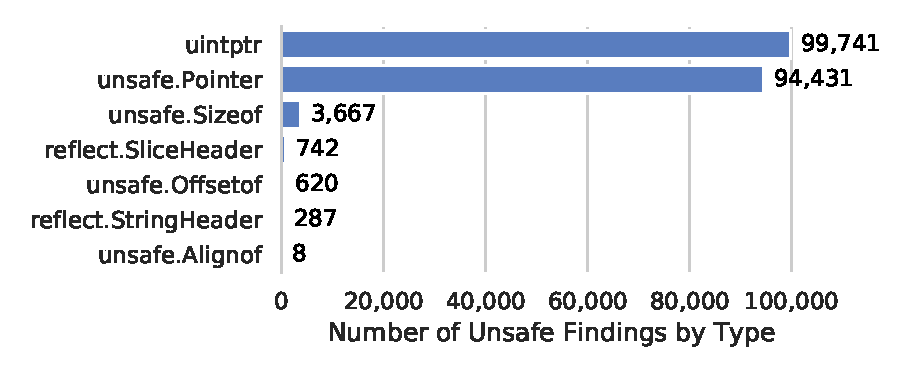
\includegraphics[width=0.43\textwidth]{assets/plots/distribution-unsafe-types.pdf}
    \caption{Distribution of different types of unsafe tokens}
    \label{fig:unsafe-tokens-distribution}
\end{figure}

We present a summary of our labeled data set consisting of \checkNum{1,400} code snippets from the \checkNum{10} projects shown in Table~\ref{tbl:dataset-projects} in Table~\ref{tbl:dataset-classes}.

\begin{table}[h]
    \centering
    \caption{Selected projects for creation of the labeled data set}
    \label{tbl:dataset-projects}
    \begin{tabular}{llrrll}
    \hline
        {}  &                                               Name &  Stars &  Forks &   Revision \\ \hline
        1   &                              kubernetes/kubernetes &  66512 &  23806 &  fb9e1946b0 \\
        2   &                       mattermost/mattermost-server &  18277 &   4157 &  e83cc7357c \\
        3   &                                    rancher/rancher &  14344 &   1758 &  56a464049e \\
        4   &                                   weaveworks/scope &   4354 &    554 &  bf90d56f0c \\
        5   &                                          rook/rook &   7208 &   1472 &  ff90fa7098 \\
        6   &                                      elastic/beats &   8852 &   3207 &  df6f2169c5 \\
        7   &                                hashicorp/terraform &  22151 &   5729 &  01f91316da \\
        8   &                                      cilium/cilium &   5501 &    626 &  9b0ae85b5f \\
        9   &                                       grafana/loki &   9537 &    922 &  10a1f28a85 \\
        10  &                                  gorgonia/gorgonia &   3373 &    301 &  5fb5944d4a \\
        \hline
    \end{tabular}
\end{table}

We select the top \checkNum{10} projects with the most unsafe usages in non-standard library packages.
These projects, including the revision that we analyzed, are shown in Table~\ref{tbl:dataset-projects}.
From these projects and all their transitive dependencies, we randomly sample \checkNum{1000} application code and \checkNum{400} standard library code snippets. We define application code as all packages that are not part of the Go standard library or the \textit{golang.org/x/sys} module, as this module contains similar abstractions and code usages as the standard library. We split the snippets to analyze whether there is a difference in use between the two.
Then, we identify class labels in two dimensions: what is being done, and for what purpose. Finally, we manually label all \checkNum{1,400} code snippets.

\begin{table*}[htp!]
    \centering
    \caption[Labeled unsafe.Pointer usages in application code (non standard library) and standard library samples]
        {Labeled unsafe.Pointer usages in application code (non standard library) and standard library samples~\newline \tiny ~\newline \footnotesize
        \underline{eff}: efficiency, \underline{ser}: (de)serialization, \underline{gen}: generics,
        \underline{no GC}: avoid garbage collection, \underline{atomic}: atomic operations,
        \underline{FFI}: foreign function interface, \underline{HE}: hide from escape analysis, \underline{layout}: memory layout control,
        \underline{types}: Go type system,
        \underline{reflect}: type reflection, \underline{unused}: declared but unused \tiny ~\newline}
    \label{tbl:dataset-classes}
    \begin{adjustbox}{max width=\textwidth}
    
    %% do not paste from notebook, local changes done!
\begin{tabular}{r|cc|cc|cc|cc|cc|cc|cc|cc|cc|cc|cc|cc}
                    & \multicolumn{2}{c|}{\textbf{eff}} & \multicolumn{2}{c|}{\textbf{ser}} & \multicolumn{2}{c|}{\textbf{gen}} & \multicolumn{2}{c|}{\textbf{no GC}} & \multicolumn{2}{c|}{\textbf{atomic}} & \multicolumn{2}{c|}{\textbf{FFI}} & \multicolumn{2}{c|}{\textbf{HE}} & \multicolumn{2}{c|}{\textbf{layout}} & \multicolumn{2}{c|}{\textbf{types}} & \multicolumn{2}{c|}{\textbf{reflect}} & \multicolumn{2}{c|}{\textbf{unused}} & \multicolumn{2}{c}{\textbf{total}} \\ %\hline
                    &  \textbf{app} &  \textbf{std} &  \textbf{app} &  \textbf{std} &  \textbf{app} &  \textbf{std} &   \textbf{app} &  \textbf{std} &    \textbf{app} &  \textbf{std} &  \textbf{app} &  \textbf{std} &  \textbf{app} &  \textbf{std} &    \textbf{app} &  \textbf{std} &   \textbf{app} &  \textbf{std} &     \textbf{app} &  \textbf{std} &    \textbf{app} &  \textbf{std} &   \textbf{app} &  \textbf{std} \\ \hline
                    
                    \textbf{cast} & 562 & 16 & 178 & 33 & 18 & & & & & & 24 & 6 && 2 & 3 & 13 & & 45 & 1 & & & & 786 & 115 \\ 
      %  cast-struct &  401 &    4 &   50 &    6 &    6 &      &       &      &        &      &    6 &    2 &      &    2 &        &    4 &       &   31 &         &      &        &      &   463 &   49 \\
%\rowcolor{verylightgray}
      %   cast-basic &   90 &    2 &   29 &    3 &    1 &      &       &      &        &      &    1 &    3 &      &      &      2 &    7 &       &    1 &         &      &        &      &   123 &   16 \\
      %  cast-header &   36 &    1 &    3 &      &    1 &      &       &      &        &      &      &      &      &      &        &      &       &    3 &         &      &        &      &    40 &    4 \\
%\rowcolor{verylightgray}
      %   cast-bytes &   22 &    1 &   81 &   11 &      &      &       &      &        &      &    1 &      &      &      &      1 &      &       &    1 &         &      &        &      &   105 &   13 \\
      % cast-pointer &   13 &    8 &   15 &   13 &   10 &      &       &      &        &      &   16 &    1 &      &      &        &    2 &       &    9 &       1 &      &        &      &    55 &   33 \\
\rowcolor{verylightgray}
      \textbf{memory-access} &    2 &    1 &    9 &      &      &      &       &      &        &      &      &    1 &      &      &      4 &    6 &       &    4 &         &      &        &      &    15 &   12 \\
 \textbf{pointer-arithmetic} &    7 &    2 &    6 &    1 &      &      &       &      &        &    1 &      &    3 &    1 &    2 &      3 &    8 &       &    9 &         &      &        &      &    17 &   26 \\
\rowcolor{verylightgray}
         \textbf{definition} &    4 &    1 &   23 &      &    2 &      &       &      &        &      &    4 &    5 &      &      &        &    9 &       &    8 &       6 &    3 &        &      &    39 &   26 \\
           \textbf{delegate} &    4 &      &   64 &      &    2 &      &       &      &     11 &    5 &   29 &   45 &      &    4 &        &   14 &       &    6 &         &    1 &        &      &   110 &   75 \\
\rowcolor{verylightgray}
            \textbf{syscall} &      &      &      &      &      &      &    17 &  138 &        &      &      &      &      &      &        &      &       &      &         &      &        &      &    17 &  138 \\
             \textbf{unused} &      &      &      &      &      &      &       &      &        &      &      &      &      &      &        &      &       &      &         &      &     16 &    8 &    16 &    8 \\ \hline
%\rowcolor{verylightgray}
                  \textbf{total} &  579 &   20 &  280 &   34 &   22 &    0 &    17 &  138 &     11 &    6 &   57 &   60 &    1 &    8 &     10 &   50 &     0 &   72 &       7 &    4 &     16 &    8 &  1000 &  400 \\
\end{tabular}

    \end{adjustbox}
        \vspace{-10pt}
\end{table*}

\jl{Todo: Include description of classes}.
We identify the following usage classes:
The most prevalent are \textit{conversion-struct-struct}, \textit{conversion-struct-basic}, \textit{conversion-header}, \textit{conversion-struct-bytes}, and \textit{conversion-pointer}, which are all cast operations from arbitrary types to other arbitrary structs, basic Go types such as \texttt{int}, slice or string headers, byte slices, or raw \texttt{unsafe.Pointer} values.
\textit{Pointer-arithmetic} denotes usages of \unsafe{} to do some form of manual arithmetic manipulation of addresses, such as advancing an array.
\textit{Definition} groups usages where a field or method of type \unsafe.Pointer{} is declared.
\textit{Delegate} are instances where \unsafe{} is only needed in a function to pass it along to another function that requires a parameter of type \texttt{unsafe.Pointer}, thus the need to use \unsafe{} is actually located somewhere else.
\textit{Type-reflection}: todo.
\textit{Syscall}: todo.
As the name suggests, \textit{unused} is a class of occurances that are not actually used.

\jl{Todo: include insights}
We see that...

Among the \checkNum{1,400} labeled snippets, \checkNum{683} are located in generated code (which means they are in a file name containing \texttt{.generated.go}, \texttt{generated\_}, \texttt{zsyscall\_}, \texttt{zz\_generated} or generated CGo file).
It might be safe to assume that generated code is less dangerous, however as bugs in the code generator can have very serious effects of scale, we include them in the study nonetheless.

\begin{tcolorbox}
Answer to \ref{rq:purpose}: Developers primarily use \unsafe{} in casting operations to improve efficiency or call CGo code or system calls.
\end{tcolorbox}